\documentclass[a4paper]{article}

\usepackage{graphicx}
\usepackage{subfig}
\usepackage{multirow}
\usepackage{amsmath}
\usepackage[utf8]{inputenc}

\graphicspath{{figuras/}}

\hyphenation{ve-ri-fi-car FalaBrasil}

\title{Relatório 02}

\author{Pedro Batista (08080002701) - pedro@ufpa.br}

\begin{document}

\maketitle

\section{Identificação Direta}

\subsection{Sistema de Primeira Ordem}\label{sec:exp1}
O esquema de simulação montado é mostrado na Figura~\ref{fig:exp}. A entrada degrau
tem amplitude 2, e a configuração \verb-A,B,C- e \verb-D- do \verb.State-Space. foi respectivamente \verb.-1,2,1. e \verb.0..

\begin{figure}[h]
   \centering
   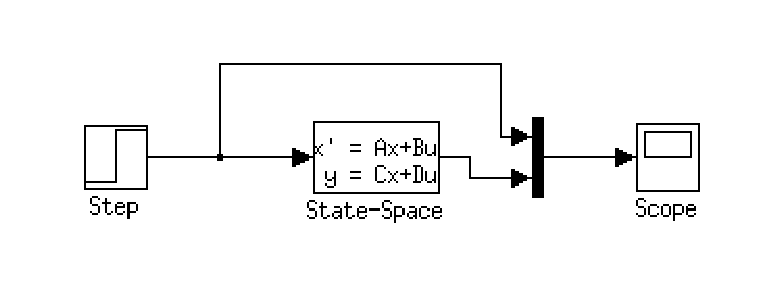
\includegraphics[width=2.5in]{exp}
   \caption{Esquema de simulação montado no Simulink.}
   \label{fig:exp}
\end{figure}

A partir do sinal de saída (mostrado na Figura~\ref{fig:exp1_simulado}) obtemos os seguintes valores:
$y(\infty)=4$ e $t_{r_{5\%}}=2.996$. A partir das seguintes equações foi possível calcular a constante
de tempo $\tau$ e o ganho do sistema \verb-k-.
$$k=\frac{y(\infty)}{U}=\frac{4}{2}=2$$
$$\tau=\frac{t_{r_{5\%}}}{3}=\frac{2.996}{3}=0.998$$

\begin{figure}[h]
   \centering
   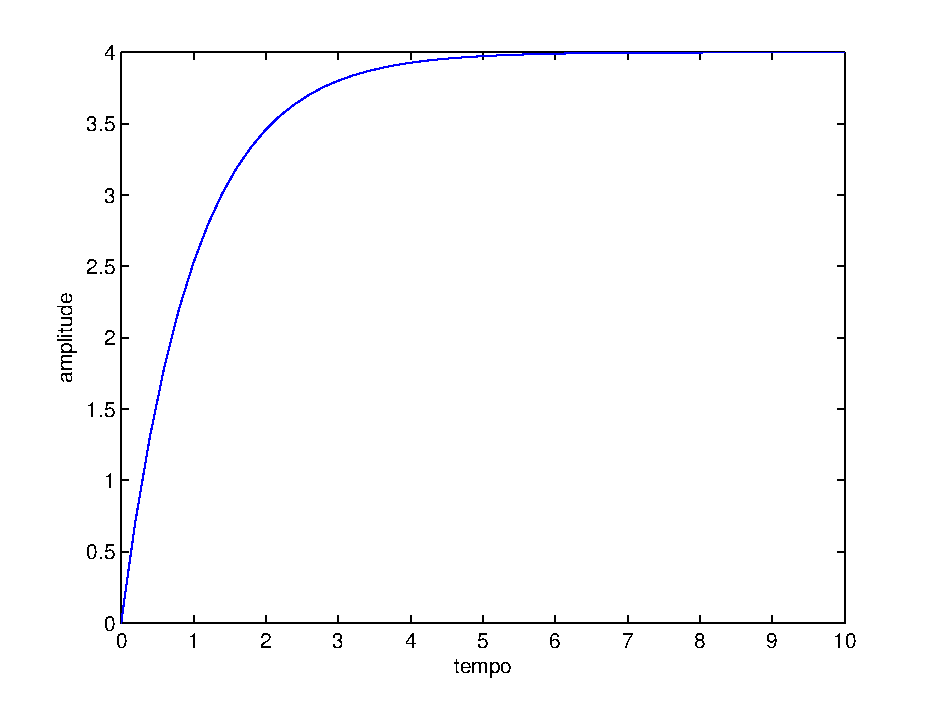
\includegraphics[width=4in]{exp1_simulado}
   \caption{Saída do controlador, montado na Seção~\ref{sec:exp1}.}
   \label{fig:exp1_simulado}
\end{figure}

\subsection{Sistema de Segunda Ordem}\label{sec:exp2}
O esquema de simulação é o mesmo utilizando para sistemas de primeira ordem (Figura~\ref{fig:exp}).
Porém a amplitude do degrau agora é 1, e a configuração do \verb.State-Space. é mostrada abaixo.
$$A=
\begin{bmatrix}
-1.824 & 2 \\
2      & 0 \\
\end{bmatrix}$$

$$B=
\begin{bmatrix}
2 \\
0 \\
\end{bmatrix}$$

$$C=
\begin{bmatrix}
0 & 1 \\
\end{bmatrix}$$

$$D=0$$

O gráfico gerado pela simulação, apresentado na Figura~\ref{fig:exp2_simulado}.
Mostra os valores de: valor de regime permanente $y(\infty)=1$; máximo sobre
sinal $M_p=0.2$ e tempo de estabilização $t_s=4.17$. A seguinte equação nos
fornece a constante de amortecimento do sistema $\xi$.
$$M_p=e^{\frac{\xi\pi}{\sqrt{1-\xi^2}}}$$
de onde obtemos:
$$\xi=\sqrt{\frac{\ln^2(M_p)}{\ln^2(M_p)+\pi^2}}$$
logo
$$\xi=\sqrt{\frac{\ln^2(0.2)}{\ln^2(0.2)+\pi^2}}=0.45594$$
Para obtenção de $w_n$ utilizamos a seguinte equação:
$$t_s=\frac{4}{\xi w_n}$$
de onde obtemos:
$$w_n=\frac{4}{\xi t_s}=\frac{4}{0.45594~4.17}=2.1038$$


\begin{figure}[h]
   \centering
   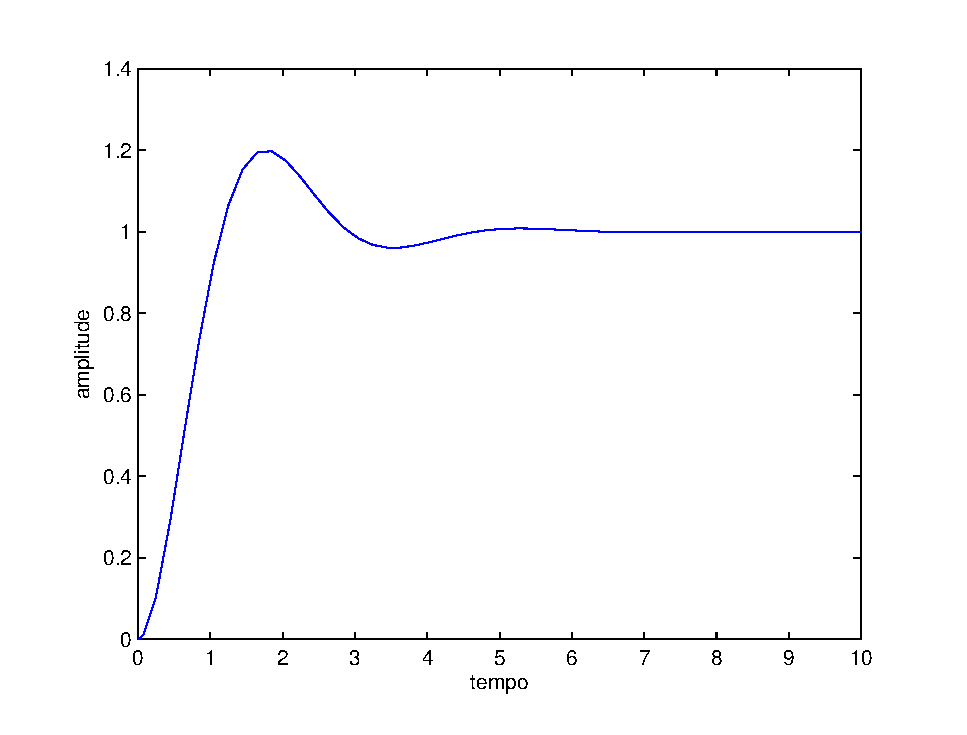
\includegraphics[width=4in]{exp2_simulado}
   \caption{Saída do controlador, montado na Seção~\ref{sec:exp2}.}
   \label{fig:exp2_simulado}
\end{figure}


\bibliographystyle{plain}
\bibliography{bib.bib} 
\end{document}
